\documentclass{beamer}

\usepackage{graphicx}
\usepackage{multicol}
\usepackage[labelfont=footnotesize,textfont=scriptsize,bf]{caption}
\usepackage{subfig}
\usepackage{siunitx}

\usepackage[utf8]{inputenc}
\usepackage[italian]{babel}
\usepackage[T1]{fontenc}

\graphicspath{{img/}}

\usetheme[hideothersubsections,width=60px]{PaloAlto}
\usecolortheme{wolverine}
\useinnertheme{rectangles}

\title[Tecnologie e opensource per i BB.CC.: il caso di Siponto (FG))]{Tecnologie e opensource applicate ai Beni Culturali per lo studio e la valorizzazione di Siponto (Manfredonia FG)}
\author[Francesco de Virgilio]{Francesco de Virgilio \\ \texttt{\tiny francesco.devirgilio@openoia.org}}
\institute[O.I.A.~Open Idea for Archaeology]{
	%\inst{1}%
	OIA --- Open Idea for Archaeology%\\
	%\emph{Università degli Studi di Bari}
	}
	% \and
	% \inst{2}%
	% School for Computational Science\\
	% Florida State University}

\pgfdeclaremask{toplogo}{oia-logo}
\pgfdeclareimage[mask=toplogo,width=1.2cm]{oia-logo}{img/oia-logo}

\logo{\vbox{\vskip0.1cm\hbox{\pgfuseimage{oia-logo}}}}


\begin{document}

\AtBeginSection[]
	{
	\begin{frame}
		\frametitle{Sommario}
		\begin{multicols}{2}
			\tableofcontents[currentsection]
		\end{multicols}
	\end{frame}
	}

\begin{frame}
	\titlepage
\end{frame}

% -----------------------------------------------------

\section*{Sommario}

	\begin{frame}{Sommario}
		\begin{multicols}{2}
			\tableofcontents
		\end{multicols}
	\end{frame}
	
\part{Gestire un progetto}
	\frame{\partpage}

	\section{Come nasce}

		\begin{frame}{Info sul progetto}
			\begin{description}
				\item[quando] 2010
				\item[chi finanzia] Regione Puglia, Bollenti Spiriti -- Principi Attivi
				\item[costo] 25000 euro
				\item[durata] il progetto è stato realizzato in 15 mesi
				\item[team] 4 archeologhe + 1
			\end{description}
			\vfill
			\begin{figure}[]
				\begin{center}
					
\includegraphics[width=0.2\linewidth]{regione}\hfill
					
\includegraphics[width=0.3\linewidth]{pa}
				\end{center}
				\label{fig:regione}
			\end{figure}
		\end{frame}

		\begin{frame}{Obiettivi}
			\begin{itemize}
				\item informatizzazione documentazione di scavo Siponto
				\item informatizzazione cartografia di scavo e rilievi
				\item implementazione webGIS archeologico
				\item realizzazione tour immersivo \SI{360}{\degree}
				\item riproduzione 3D di 10 reperti significativi
				\item tutti i dati devono essere presentati ed interrogabili via web per mezzo di apposite interfacce
				\item realizzazione esclusivamente con Software Libero
			\end{itemize}
		\end{frame}

	\section{L'importanza della progettazione}
		
		\begin{frame}{Scrittura}
			\begin{itemize}
				\item 2 mesi di ricerche
				\item 2 mesi per scrivere il progetto
				\item 5 persone
				\item diversi test sulle tecnologie
			\end{itemize}
		\end{frame}

		\begin{frame}{Regole auree}
			\begin{description}
				\item[idee chiare] cambiare idea su alcuni punti del progetto può essere difficile o impossibile in corso d'opera, meglio definire alcuni concetti all'inizio e non cambiarli
				\item[non procastinare] non rimandare al momento della realizzazione ciò che può essere pianificato prima, potrebbero insorgere ulteriori problemi
				\item[essere specifici] progettare significa scrivere le \emph{specifiche} del progetto, ovvero numeri, grafi, passaggi e modalità di implementazione nei particolari
				\item[il tempo] c'è tutto il tempo che serve, ma non è mai abbastanza; non sottovalutare l'importanza delle date: creare delle deadline e seguirle.
			\end{description}
		\end{frame}

		\begin{frame}{Hai un piano B?}

			\begin{block}{Quarta legge della termodinamica}
				\emph{Se qualcosa può andare male, lo farà.}\\\flushright{(cit. Capt. Ed Murphy)}
			\end{block}

			\begin{itemize}
				\item per ogni punto/tecnologia, calcolare un'alternativa
				\item non ridursi all'ultimo giorno disponibile
				\item quando si dipende da servizi/prestazioni esterne, seguire minuziosamente l'avanzamento dei lavori
				\item non riporre eccessiva fiducia nei servizi della PA
			\end{itemize}
		\end{frame}

	\section{Contatti con l'estero}

		\subsection{Alla ricerca delle idee migliori}

			\begin{frame}{Guardarsi intorno, prima di tutto}
				\begin{description}
					\item[problema] sorge necessità di un sistema di gestione del dato archeologico con interfaccia web per l'inserimento dati, la visualizzazione e l'interrogazione del database
				\end{description}

				\begin{enumerate}
					\item progetto software (tempo impiegato: 1 settimana)
					\item presento il progetto in mailing list internazionali
					\item risposta: già stato realizzato (ARK)
					\item cambio il progetto per includere ARK
				\end{enumerate}
			\end{frame}

			\begin{frame}{We can do it better}
				\begin{enumerate}
					\item chiedo in mailing list internazionale
					\item risposta: esiste ARK
					\item includo ARK nel mio progetto
					\item tempo impiegato: 2 giorni
				\end{enumerate}
			\end{frame}

		\subsection{Collaborazione diretta}

			\begin{frame}{Non perdere il filo}
				Collaborare costantemente con altri enti, ricercatori, professionisti e semplici utenti aiuta a non commettere errori grossolani e velocizza l'implementazione del progetto.

				\begin{figure}
					\centering
					\subfloat[]{\label{fig:uniba}
\includegraphics[trim=0 220 0 0,clip=true,width=0.24\textwidth]{uniba}}\hfill
					\subfloat[]{\label{fig:unifg}
\includegraphics[width=0.26\textwidth]{unifg}}\hfill
					\subfloat[]{\label{fig:dicar}
\includegraphics[width=0.23\textwidth]{dicar}}\\
					\subfloat[]{\label{fig:lp}
\includegraphics[width=0.45\textwidth]{lp}}
					\caption[]{Le collaborazioni di O.I.A.}
					\label{fig:collab}
				\end{figure}
			\end{frame}

	\section{Sperimentazione e software libero}
		
		\begin{frame}{Sperimentazione: alcune accortezze}
			I progetti sono finanziati in base al grado di innovazione: ecco alcuni rischi.
			\begin{itemize}
				\item i progetti sperimentali, per quanto possano essere pianificati, sono spesso suscettibili di ritardi dovuti ad errori tecnici, inesperienza o imprevisti
				\item prove durante la progettazione: non indispensabili ma consigliate
				\item in ambito software libero, indispensabile collaborare con comunità online
			\end{itemize}
		\end{frame}

		\begin{frame}{Cos'è il software libero}
			Secondo Richard Stallman e la Free Software Foundation da lui fondata, un software si può definire libero solo se garantisce quattro ``libertà fondamentali'':
			\begin{description}
				\item[Libertà 0] Libertà di eseguire il programma per qualsiasi scopo.
				\item[Libertà 1] Libertà di studiare il programma e modificarlo.
				\item[Libertà 3] Libertà di ridistribuire copie del programma in modo da aiutare il prossimo.
				\item[Libertà 4] Libertà di migliorare il programma e di distribuirne pubblicamente i miglioramenti, in modo tale che tutta la comunità ne tragga beneficio.
			\end{description}
		\end{frame}

		\begin{frame}{Cosa abbiamo usato}
			\vspace{-30px}
			\begin{figure}
				\subfloat[]{
\includegraphics[width=0.2\textwidth]{sw_logos/bootstrap}}\hfill
				\subfloat[]{
\includegraphics[width=0.2\textwidth]{sw_logos/apache}}\hfill
				\subfloat[]{
\includegraphics[width=0.2\textwidth]{sw_logos/ark}}\hfill
				\subfloat[]{
\includegraphics[trim=0 75 0 10,clip=true,width=0.2\textwidth]{sw_logos/gimp}}\\
				\subfloat[]{
\includegraphics[width=0.2\textwidth]{sw_logos/hugin}}\hfill
				\subfloat[]{
\includegraphics[width=0.2\textwidth]{sw_logos/jinja}}\hfill
				\subfloat[]{
\includegraphics[width=0.2\textwidth]{sw_logos/jquery}}\hfill
				\subfloat[]{
\includegraphics[width=0.2\textwidth]{sw_logos/mapiscons}}\\
				\subfloat[]{
\includegraphics[width=0.2\textwidth]{sw_logos/mapserver}}\hfill
				\subfloat[]{
\includegraphics[width=0.2\textwidth]{sw_logos/ol}}\hfill
				\subfloat[]{
\includegraphics[width=0.1\textwidth]{sw_logos/osm}}\hfill
				\subfloat[]{
\includegraphics[width=0.2\textwidth]{sw_logos/python}}\\
				\subfloat[]{
\includegraphics[width=0.2\textwidth]{sw_logos/thingiview}}\hfill
				\subfloat[]{
\includegraphics[width=0.2\textwidth]{sw_logos/timelinejs}}\hfill
				\subfloat[]{
\includegraphics[width=0.2\textwidth]{sw_logos/ubuntu}}\hfill
				\subfloat[]{
\includegraphics[width=0.2\textwidth]{sw_logos/webgl}}\hfill
			\end{figure}
		\end{frame}

		\begin{frame}{Cosa abbiamo usato}
			\vspace{-30px}
			\begin{figure}
				\subfloat[]{
\includegraphics[width=0.2\textwidth]{sw_logos/phpmyadmin}}\hfill
				\subfloat[]{
\includegraphics[width=0.2\textwidth]{sw_logos/meshlab}}\hfill
				\subfloat[]{
\includegraphics[width=0.2\textwidth]{sw_logos/phppgadmin}}\\\
				\subfloat[]{
\includegraphics[width=0.2\textwidth]{sw_logos/pg}}\hfill
				\subfloat[]{
\includegraphics[width=0.2\textwidth]{sw_logos/grass}}\hfill
				\subfloat[]{
\includegraphics[width=0.2\textwidth]{sw_logos/qgis}}\hfill
				\subfloat[]{
\includegraphics[width=0.2\textwidth]{sw_logos/oj}}\hfill
			\end{figure}
		\end{frame}

		\begin{frame}{Punti di vista}
			\begin{block}{Vantaggi}
				\begin{itemize}
					\item costo licenze software: 0 euro
					\item flessibile, modificabile, adattabile
					\item forte comunità di supporto: forum, chat, manuali
					\item \emph{scriptabile}
					\item sviluppato da importanti università e centri di ricerca in tutto il mondo
					\item eticamente corretto, sprona alla collaborazione
				\end{itemize}
			\end{block}
			\begin{block}{Svantaggi}
				\begin{itemize}
					\item curva di apprendimento ripida
					\item abilità nel problem solving
					\item comunità di supporto fortemente anglo-centrica
				\end{itemize}
			\end{block}
		\end{frame}

		\begin{frame}{Sviluppato collaborativamente}
			\begin{center}
				\url{https://github.com/fradeve/ark-oia}
			\end{center}
		\end{frame}

\part{www.sipontomedievale.it}
\frame{\partpage}

	\section{Generalità}

		\begin{frame}{Screenshot}
			\begin{figure}[]
				\begin{center}
					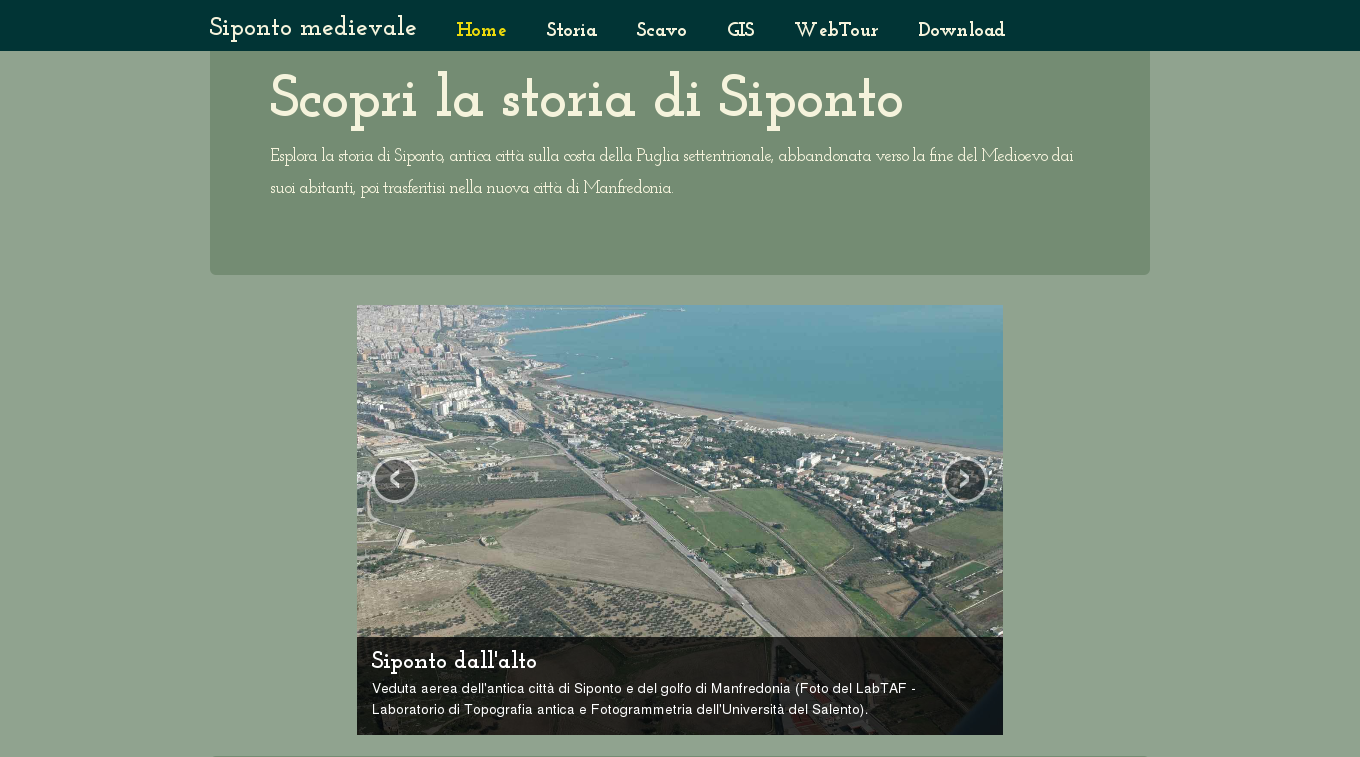
\includegraphics[width=1\linewidth]{screen_sip}
				\end{center}
				\caption{La homepage di Siponto Aperta}
				\label{fig:sip_screen}
			\end{figure}
		\end{frame}

		\begin{frame}{Caratteristiche}
			\begin{multicols}{2}[][]
				Caratteristiche:
				\begin{itemize}
					\item sviluppato con Twitter Bootstrap
					\item fruibile anche da tablet
					\item scritto in HTML, JavaScript, AJAX
					\item contiene materiali scaricabili (brochure, carta archeologica)
					\item contenuti multimediali (JavaScript, HTML5)
				\end{itemize}
				\columnbreak
				Sezioni principali:
				\begin{itemize}
					\item Home
					\item Storia
					\item Scavo
					\item GIS
					\item WebTour
					\item Download
				\end{itemize}
			\end{multicols}
		\end{frame}

		\begin{frame}{Struttura}
			\begin{figure}[]
				\begin{center}
					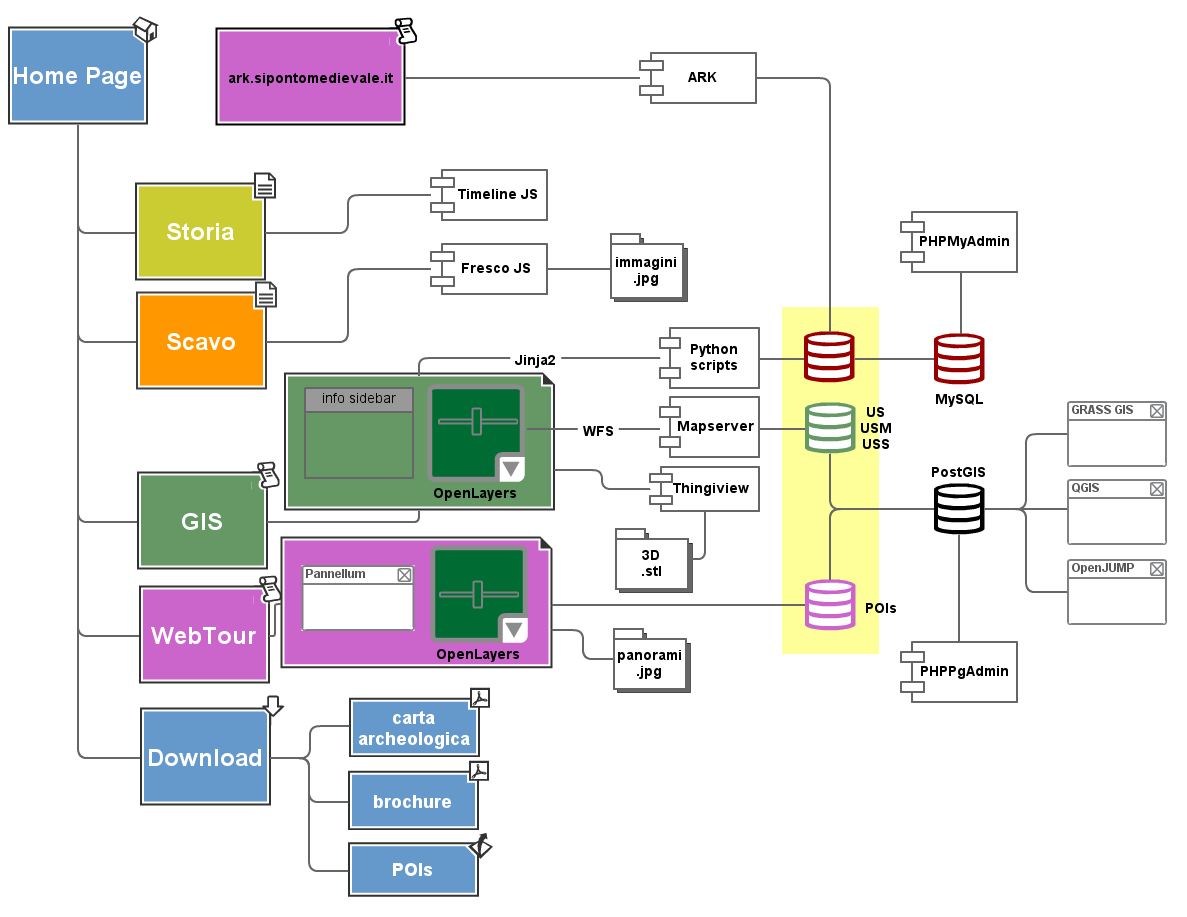
\includegraphics[width=1.0\linewidth,trim=7 20 20 20,clip=true]{struct}
				\end{center}
				\label{fig:struct}
			\end{figure}
		\end{frame}

	\section{Multimedialità}

		\begin{frame}{La linea del tempo}
			\begin{figure}[]
				\begin{center}
					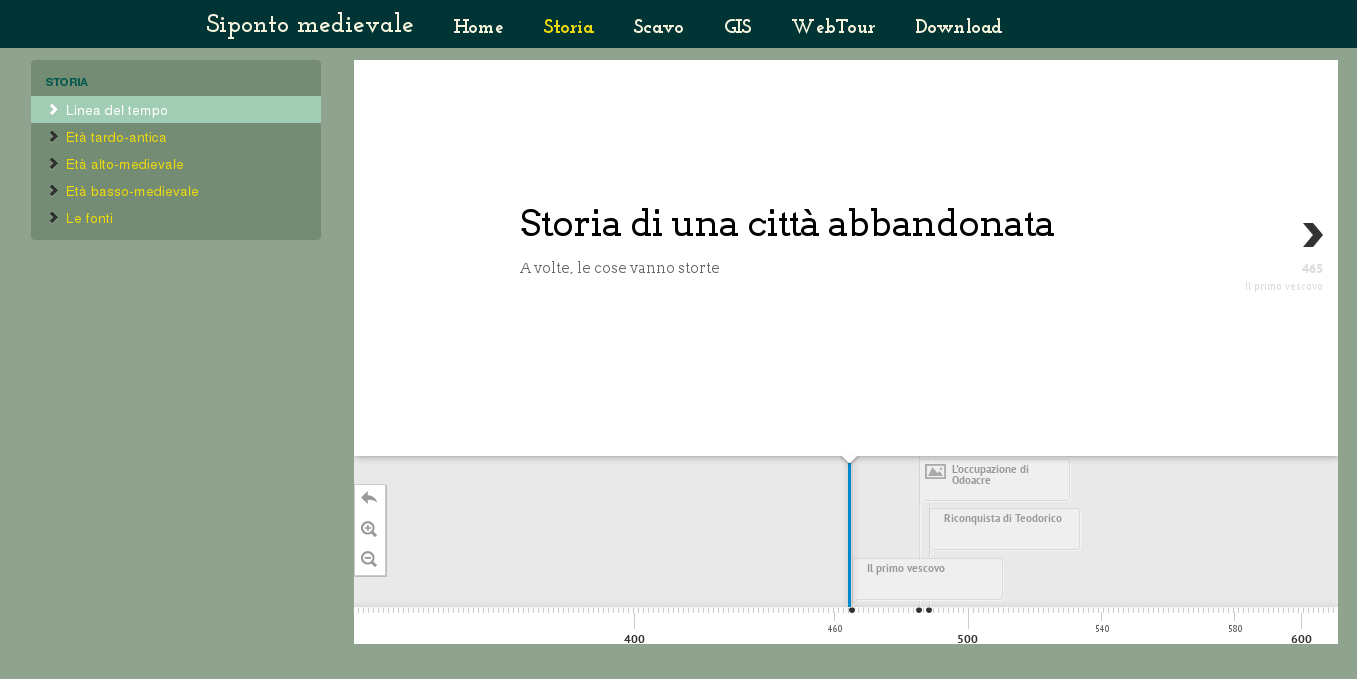
\includegraphics[width=1\linewidth]{timeline}
				\end{center}
				\label{fig:timeline}
			\end{figure}
			Realizzata con Timeline JS e tanta, tanta pazienza.\\
			\begin{center}\url{www.sipontomedievale.it/story.html}\end{center}
		\end{frame}

		\begin{frame}{Gallerie}
			\begin{figure}[]
				\begin{center}
					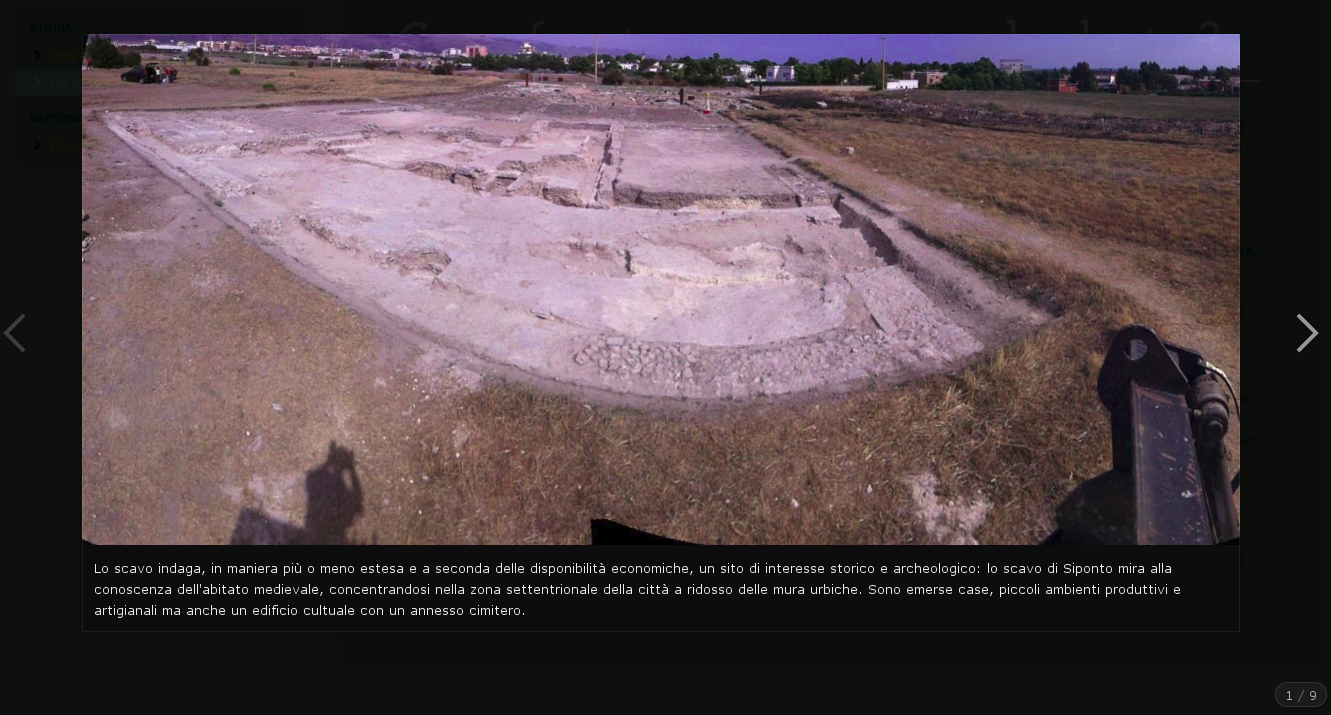
\includegraphics[width=1\linewidth]{gallery}
				\end{center}
				\label{fig:gallery}
			\end{figure}
			Realizzate con FrescoJS\\
			\centering
			\begin{center}\url{www.sipontomedievale.it/dig.html}\end{center}
		\end{frame}

		\begin{frame}{WebTour immersivo}
			\begin{figure}[]
				\begin{center}
					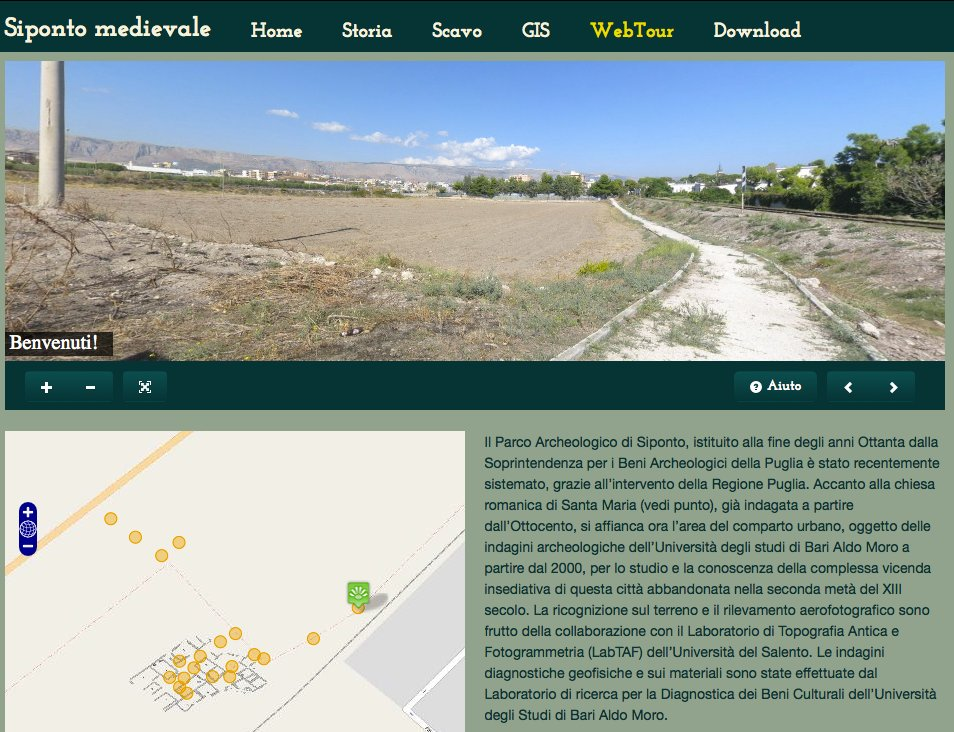
\includegraphics[width=0.75\linewidth]{screen_tour}
				\end{center}
				\label{fig:gallery}
			\end{figure}
			Realizzato con Pannellum, OpenLayers, JavaScript, AJAX\\
			\centering
			\begin{center}\url{www.sipontomedievale.it/tour.html}\end{center}
		\end{frame}

\part{Siponto Aperta: documentazione archeologica}
\frame{\partpage}

	\section{Documentazione tradizionale}

		\begin{frame}{La scheda di US cartacea}
			\begin{multicols}{2}[][]
				\begin{figure}[]
					\begin{center}
						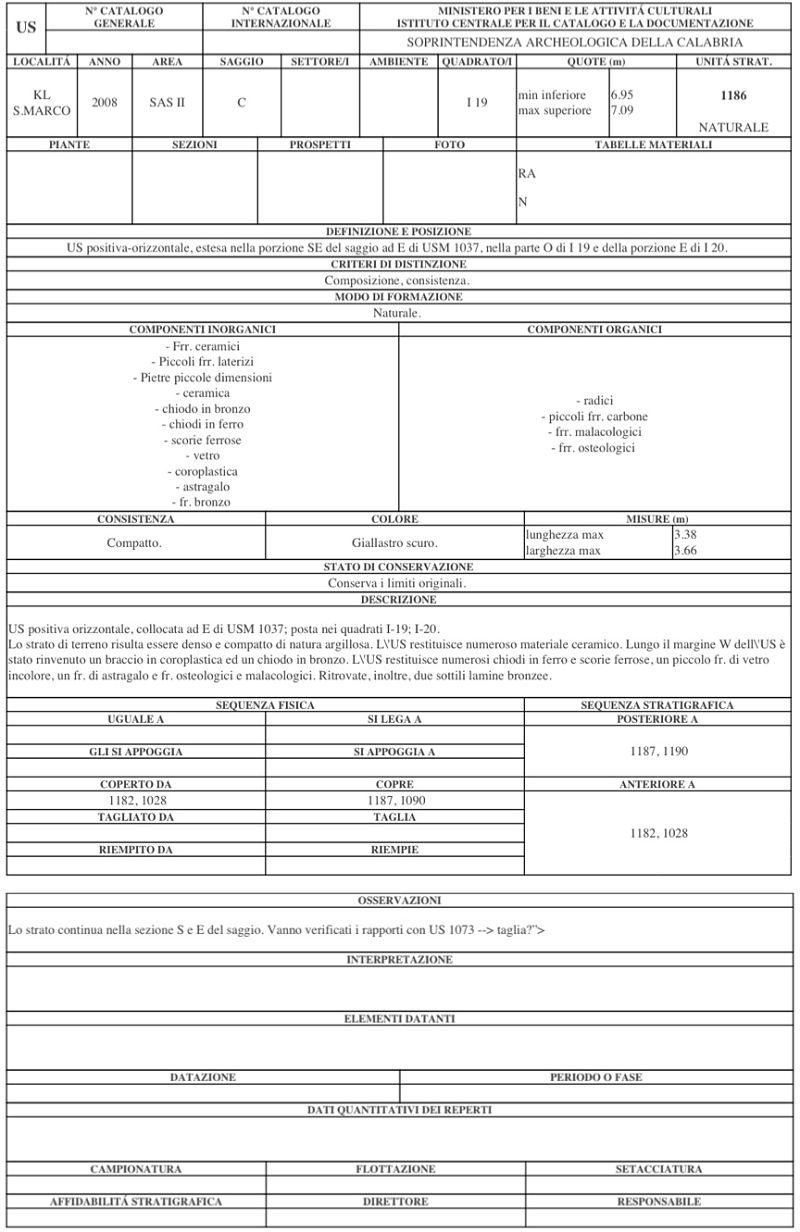
\includegraphics[width=0.9\linewidth]{us}
					\end{center}
					\caption{Scheda US italiana}
					\label{fig:us}
				\end{figure}
				\columnbreak
				Interessante caso di documentazione che presenta quasi solo \emph{svantaggi}:
				\begin{itemize}
					\item difficoltà di gestione: spazi, volumi, ingombro
					\item incrocio di informazioni quasi impossibile
					\item difficile ampliare i campi informativi
					\item difficile trasmettere le informazioni, comunicarle, farne un backup
				\end{itemize}
			\end{multicols}
		\end{frame}

		\begin{frame}{Il labirinto dei database archeologici}
			Pensare che la scelta di un database archeologico sia semplice, è un errore
			\begin{itemize}
				\item assenza completa di standard
				\item ogni tipologia di dato necessità di una differente struttura di db
				\item tanti casi di studio, molto differenti tra loro
				\item poche soluzioni ``precotte''
				\item aumento dei dati/tipologie di dati = aumento della complessità
				\item scelta del db: e se poi te ne penti?
			\end{itemize}
		\end{frame}

		\begin{frame}{Pentimenti}
			La scelta errata di un database, della sua struttura ed organizzazione può compromettere seriamente tutto \emph{postprocessing} dei dati di scavo: interrogazione, analisi, studio, gestione.
		\end{frame}

		\begin{frame}{Casi interessanti}
		\framesubtitle{Lista non completa}
			\begin{description}
				\item[iadb]\emph{Integrated Archaeological Database}\\University of Reading, Southampton, Nottingham, Salford, UCL; open source. \url{http://www.iadb.org.uk/}
				\item[OpenArcheo]\\LIAAM -- Laboratorio di Informatica Applicata all'Archeologia Medievale, Università di Siena\footnote{Impossibile trovare codice sorgente/demo funzionante.}.
				\item[Microsoft Access]Soluzioni personalizzate create da aziende e laboratori; difficilmente gestibili, poco documentate.
				\item[Ark]\emph{Archeological Recording Kit}\\L.-P. Archaeology; open source. \url{http://ark.lparchaeology.com}
			\end{description}
		\end{frame}

		\begin{frame}{Criteri di scelta}
			In ordine di importanza:
			\begin{enumerate}
				\item open source, possibilmente \emph{free software}
				\item basato su standard informatici (anche \emph{de-facto})
				\item ben documentato
				\item flessibile
			\end{enumerate}
		\end{frame}

		\begin{frame}{Perché no?}
		\framesubtitle{Le ragioni degli esclusi}
			\begin{multicols}{2}[][]
				OpenArcheo
				\begin{itemize}
					\item impossibile reperire il codice sorgente
					\item non esiste demo funzionante
					\item scarsa documentazione
				\end{itemize}
				\columnbreak
				Microsoft Access
				\begin{itemize}
					\item difficoltà di esportare dati su web
					\item non open source
					\item non compatibile con sistemi Linux
				\end{itemize}
			\end{multicols}
		\end{frame}

	\section{Ark}

		\begin{frame}{Generalità}
			\begin{description}
				\item[nascita] circa 2005
				\item[basato su] PHP, MySQL, JavaScript/AJAX
				\item[sviluppato da] L.-P. Archaeology, Londra
				\item[casi eccellenti] Chersonesos (Ucraina), FASTI Online\\Portus (Roma), Prescott Street (Londra)\\Thames Discovery Program (Londra)\\Villa Magna (Chieti)
				\item[documentazione] \url{http://ark.lparchaeology.com/wiki}
				\item[comunità] mailing list utenti (\href{http://groups.google.com/group/arkusers}{Google Groups arkusers})\\sviluppatori (\href{http://groups.google.com/group/arkdev}{Google Groups arkdev})
			\end{description}
		\end{frame}

		\begin{frame}{Caratteristiche}
			\begin{figure}[]
				\begin{center}
					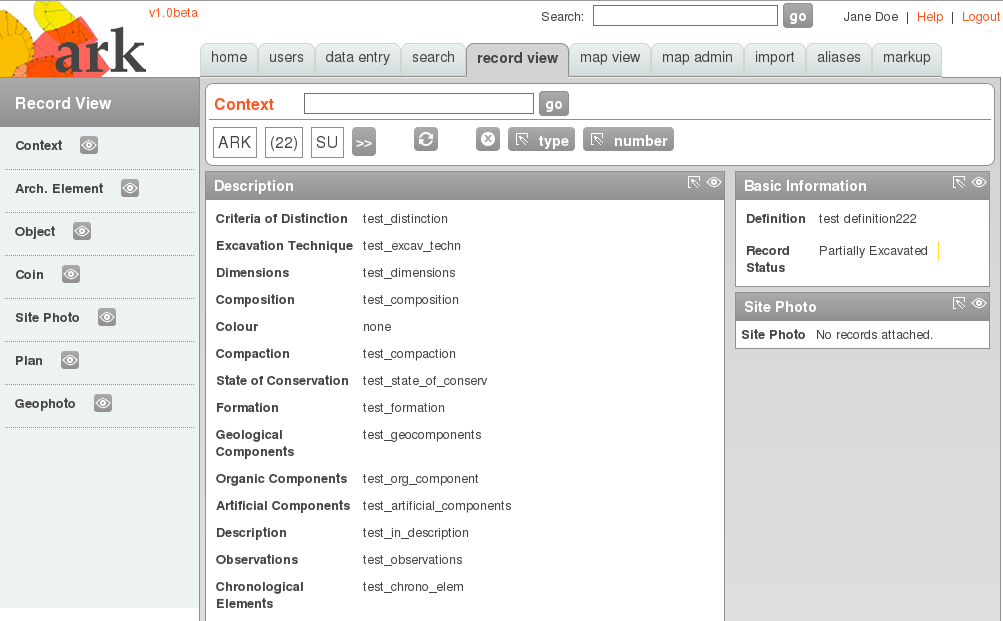
\includegraphics[width=0.7\linewidth]{screen_ark}
				\end{center}
				\label{fig:screen_ark}
			\end{figure}
			\begin{itemize}
				\item funziona su server Windows, Linux, OSX
				\item colleziona qualsiasi tipo di informazione:
					\begin{itemize}
						\item schede US, USM, USS
						\item fotografie
						\item dati spaziali (shp, dxf)
						\item database MySQL (supporto, documentazione, script)
						\item non è prestrutturato: struttura a \emph{post-it}
					\end{itemize}
			\end{itemize}
		\end{frame}

		\begin{frame}{La struttura a \emph{post-it}}
			\begin{description}
				\item[perchè]la struttura del db archeologico è una approssimazione della realtà (stratigrafia)
				\item[problema]nel tentativo di essere aderenti alla realtà, i db risultano pesanti, complessi e con troppi campi rispetto all'utilizzo medio (insieme di tabelle con tutte le possibili sfaccettature della realtà)
				\item[soluzione]definire solo l'essenziale, permette di \emph{incollare} le restanti informazioni all'occorrenza, in un albero espandibile (potenzialmente) all'infinito: struttura ad \emph{oggetti} e \emph{frammenti}
				\item[termini specialistici] \emph{docuverse} (tutti i dati sono scritti una volta sola, senza ripetizioni), \emph{transclusione}
			\end{description}
		\end{frame}

		\begin{frame}{La struttura a \emph{post-it}}
			\begin{figure}[]
				\begin{center}
					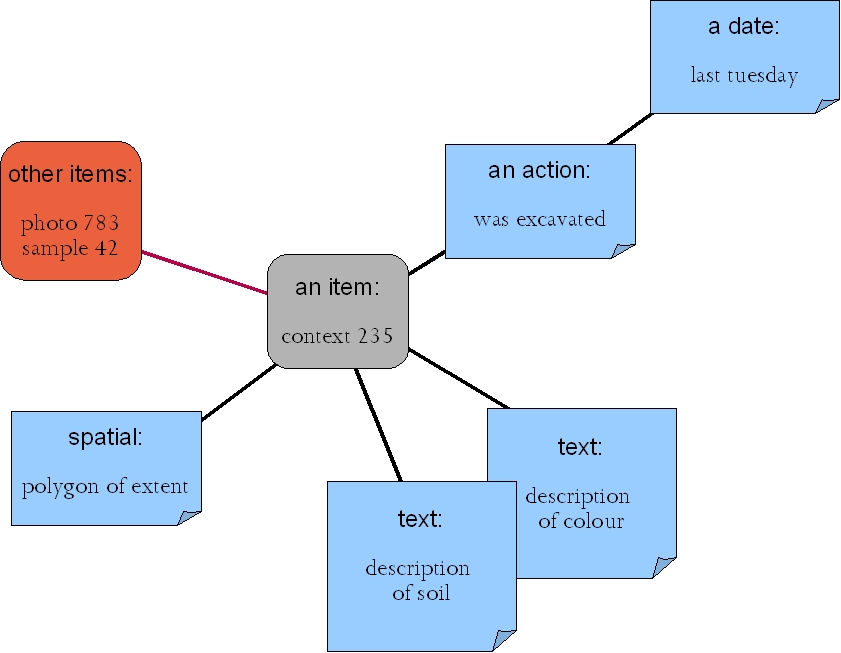
\includegraphics[width=0.8\linewidth]{ark_struct}
				\end{center}
				\caption{Struttura minima in Ark: ad ogni \emph{oggetto} vengono attaccati dei \emph{frammenti}, in un processo espandibile all'infinito (da S. Eve, G.  Hunt, \emph{ARK : A Development Framework for Archaeological Recording}, CAA 2007 proceedings).}
				\label{fig:ark_struct}
			\end{figure}
		\end{frame}

		\begin{frame}{Demo funzionante}
			\centering
			\LARGE{\url{http://ark.sipontomedievale.it}}
		\end{frame}

\part{Siponto Aperta: GIS}
\frame{\partpage}

	\section{I GIS in archeologia}
		\begin{frame}{Stratigrafia e geografia}
			In archeologia stratigrafica, il dato è strettamente legato alla geografia; le testimonianze sono localizzabili nel tempo e nello spazio:
			\begin{multicols}{2}[][]
				Documentazione
				\begin{itemize}
					\item posizione degli strati rispetto ad altri strati
					\item posizione degli strati rispetto agli ambienti
					\item posizione degli ambienti nello scavo e dello scavo nel territorio
				\end{itemize}
				\columnbreak
				Analisi
				\begin{itemize}
					\item analisi irraggiamento solare
					\item sovrapposizione LIDAR
					\item statistica di base
					\item archeologia quantitativa
				\end{itemize}
			\end{multicols}
		\end{frame}

		\begin{frame}{Analisi archeologica 1}
			\begin{figure}[]
				\begin{center}
					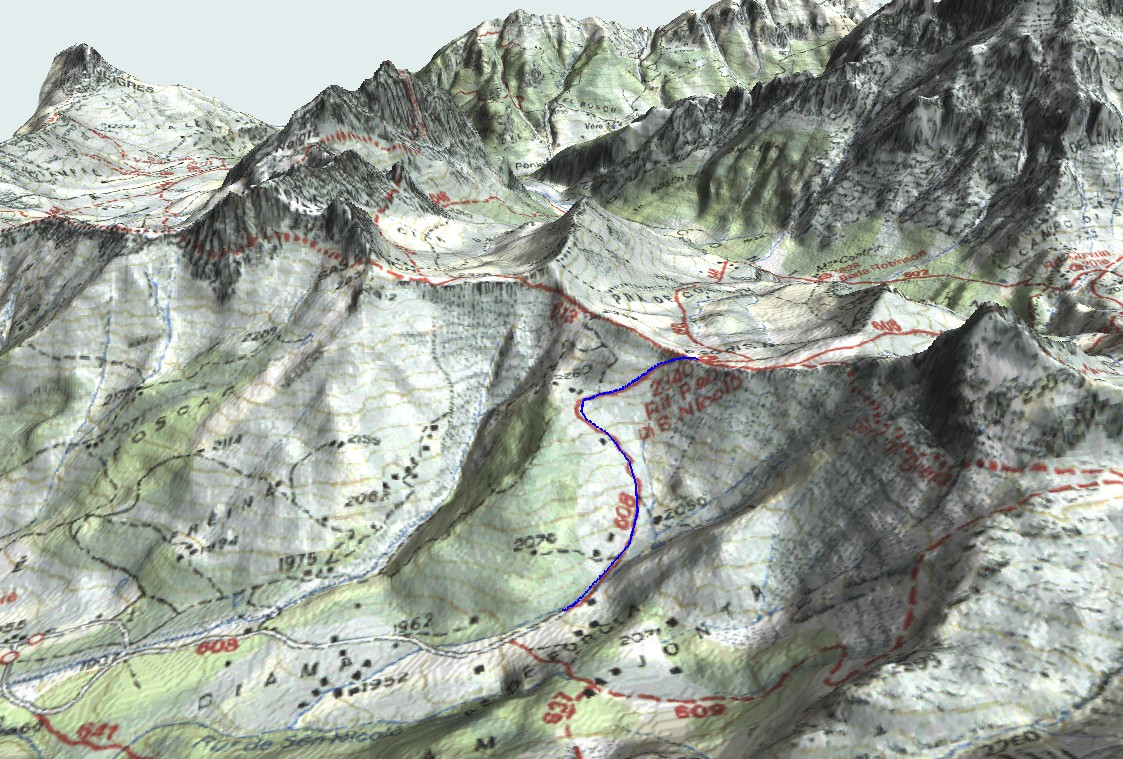
\includegraphics[width=1\linewidth]{rwalk}
				\end{center}
				\caption{\textsc{r.walk} in Val di Fassa; sentieri rossi: percorsi esistenti, sentieri verdi: calcolati; M. Franchi, “Young researchers wanted” award (PBZ, 2006)}
				\label{fig:rwalk}
			\end{figure}
		\end{frame}

		\begin{frame}{Analisi archeologica 2}
			\begin{figure}[]
				\begin{center}
					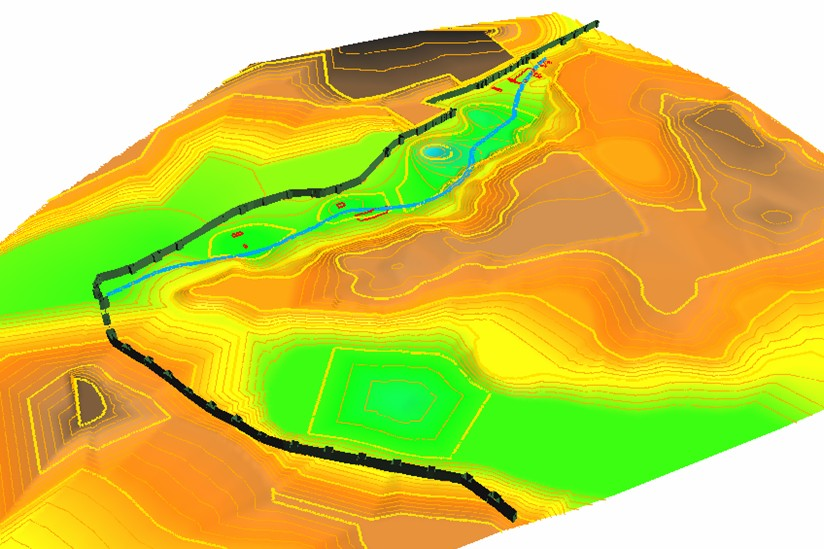
\includegraphics[width=1\linewidth]{demetr}
				\end{center}
				\caption{Ricostruzione della Marrana di San Giovanni, Roma; E. Demetrescu}
				\label{fig:demetr}
			\end{figure}
		\end{frame}

		\begin{frame}{Analisi archeologica 3}
			\begin{figure}[]
				\begin{center}
					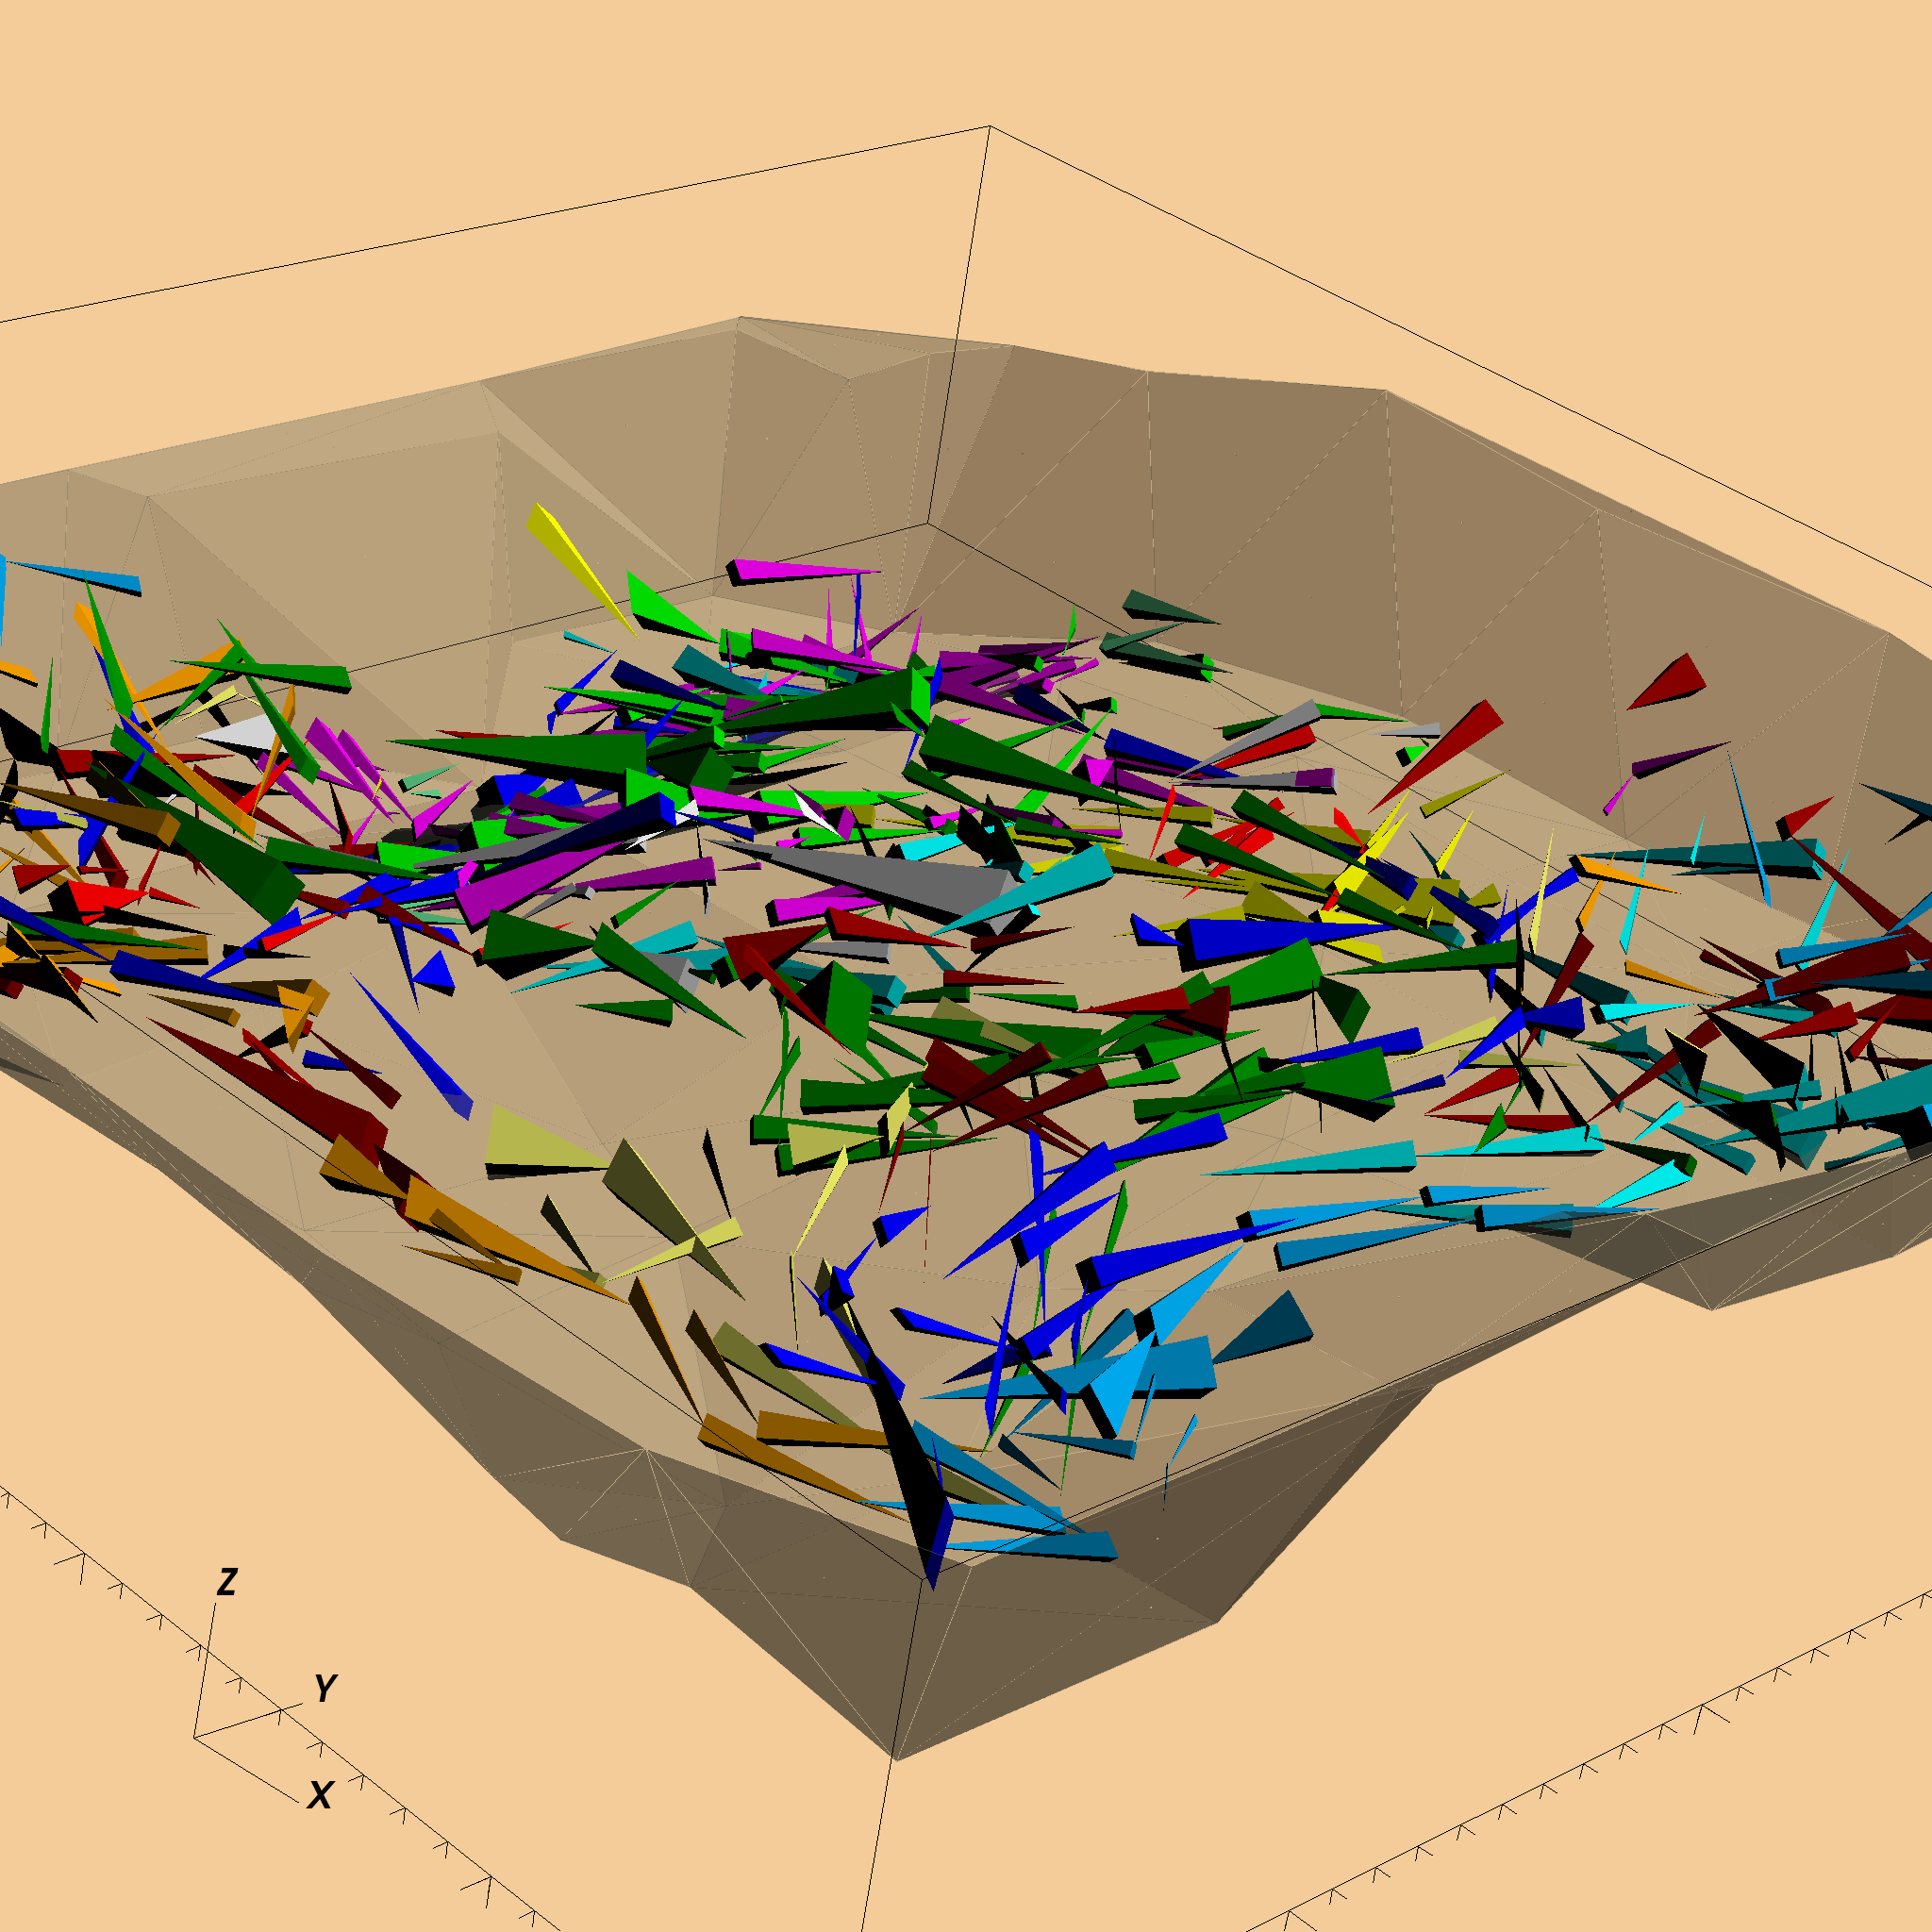
\includegraphics[width=0.65\linewidth]{oa}
				\end{center}
				\caption{Analisi posizione di ossa umane in fossa comune, Regno Unito; Benjamin Ducke, Oxford Archaeology Digital}
				\label{fig:oa}
			\end{figure}
		\end{frame}

	\section{GIS vs CAD: digitalizzazione}

		\begin{frame}{CAD: perché no?}
			\begin{block}{Spiegami perché non dovrei usare il CAD}
				Perché la Terra è tonda!
			\end{block}
			\begin{multicols}{2}[][]
				Altri buoni motivi:
				\begin{itemize}
					\item il dwg non è uno standard
					\item esistono pochi software CAD open source
					\item esportazione con perdita di dati
					\item la terra non è piatta
				\end{itemize}
				\columnbreak
				\begin{figure}[]
					\begin{center}
					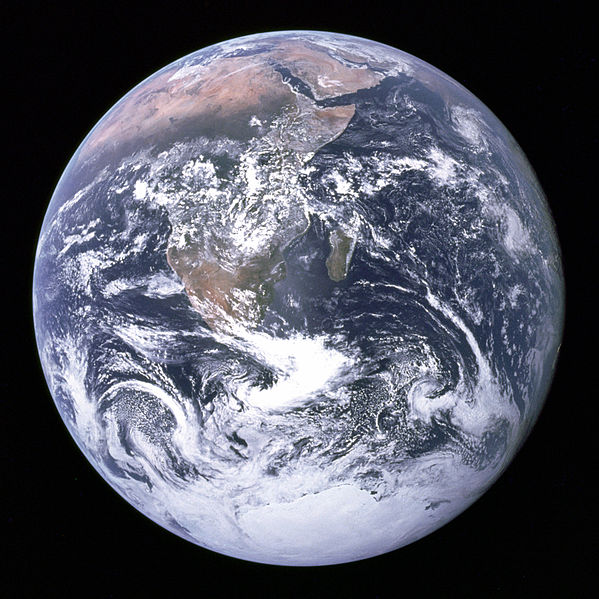
\includegraphics[width=1\linewidth]{earth}
					\end{center}
					\caption{La Terra è un geoide (credits: en.wikipedia/wiki/Earth)}
					\label{fig:earth}
				\end{figure}
			\end{multicols}
		\end{frame}

		\begin{frame}{GIS}
			\begin{center}
				Un \emph{Geographic information system} (acronimo: GIS) è un sistema adatto per catturare, immagazzinare, manipolare, analizzare, gestire e rappresentare tutti i tipi di dati geografici.\vfill
				In termini semplici, col GIS si possono unire cartografie, eseguire analisi statistiche e gestire i dati attraverso tecnologie database.
				\flushright{cit. Wikipedia}
			\end{center}
		\end{frame}

		\begin{frame}{Digitalizzazione}
			\begin{enumerate}
				\item pulizia dei dwg usando \textbf{AutoCAD}
				\begin{itemize}
					\item eliminazione di qualsiasi entità non presente nella realtà
					\item chiusura delle polilinee
					\item tempo totale: 5 giornate lavorative, 3 persone
				\end{itemize}
				\item esportazione in \emph{shapefile}
				\hline
				\item \textbf{QGIS}, sovrapposizione con carta BB.CC. SIT Puglia 
				\hline
				\item \textbf{GRASS}, georeferenziazione / riproiezione vettoriale
				\item ripetizione delle operazioni per US -- USM -- USS
				\hline
				\item \textbf{OpenJump}, pulizia e controllo shapefiles
				\hline
				\item \textbf{QGIS}, importazione altri layer dati
				\begin{itemize}
					\item ortofoto b/n (raster)
					\item prospezioni georadar (raster)
					\item layer stradale OpenStreetMap (vettoriale)
				\end{itemize}
				\item caricamento su server PostGIS
			\end{enumerate}
		\end{frame}

	\section{Un passo avanti: PostGIS}

		\begin{frame}{PostGIS e analisi}
			\begin{block}{Cos'è}
				PostGIS è un software, solitamente installato su un server, che permette di organizzare, gestire ed interrogare un database geografico.
			\end{block}
			\begin{multicols}{2}[][]
				\begin{itemize}
					\item basato su PostgreSQL
					\item gestisce raster e vettoriali
					\item integrato con QGIS, GRASS, OpenJump
					\item interfaccia web: PHPPgSQL
				\end{itemize}
				\columnbreak
				\begin{figure}[]
					\begin{center}
						
\includegraphics[width=1\linewidth]{sw_logos/pg}
					\end{center}
					\label{fig:pg_logo}
				\end{figure}
			\end{multicols}
		\end{frame}

		\begin{frame}{Struttura GIS}
			\begin{figure}[]
				\begin{center}
					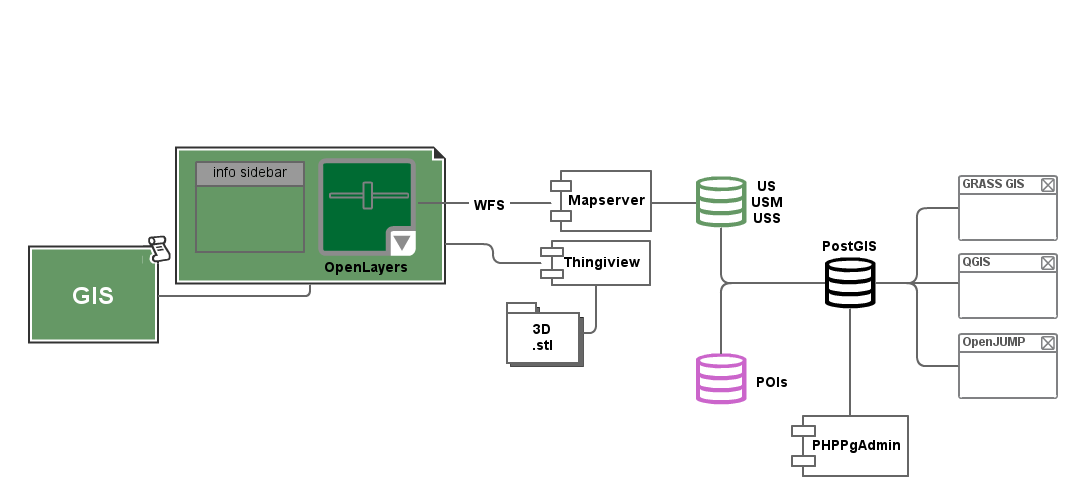
\includegraphics[width=1\linewidth,trim=20 0 0 50,clip=true]{gis_scheme}
				\end{center}
				\caption{Struttura del sistema per la gestione e visualizzazione dei dati geografici di www.sipontoaperta.it}
				\label{fig:gis}
			\end{figure}
		\end{frame}

	\section{WebGIS}

		\begin{frame}{OpenLayers}
			\begin{block}{Cos'è}
				È un software per la visualizzazione di mappe interattive interattive sul web.
			\end{block}
			\begin{multicols}{2}[][]
				\begin{itemize}
					\item scritto in Javascript
					\item altamente configurabile
					\item conforme agli standard OSGeo
				\end{itemize}
				\columnbreak
				\begin{figure}[]
					\begin{center}
					
\includegraphics[width=1\linewidth]{sw_logos/ol}
					\end{center}
					\label{fig:ol}
				\end{figure}
			\end{multicols}
			
		\end{frame}

		\begin{frame}{Come funziona una richiesta geografica}
			\begin{enumerate}
				\item l'utente seleziona un layer dalla barra in basso (US -- USM -- USS)
				\item OpenLayers prende nota del nome del layer richiesto e gira la richiesta a MapServer
				\item MapServer si collega al database PostGIS ed estrapola i dati richiesti
				\item MapServer organizza i dati in un pacchetto di informazioni geografiche (WFS) e lo invia ad OpenLayers
				\item OpenLayers visualizza WFS ricevuti e si mette in attesa di ulteriori input
			\end{enumerate}
		\end{frame}

		\begin{frame}{Screenshot webGIS con informazioni US}
			\begin{figure}[]
				\begin{center}
					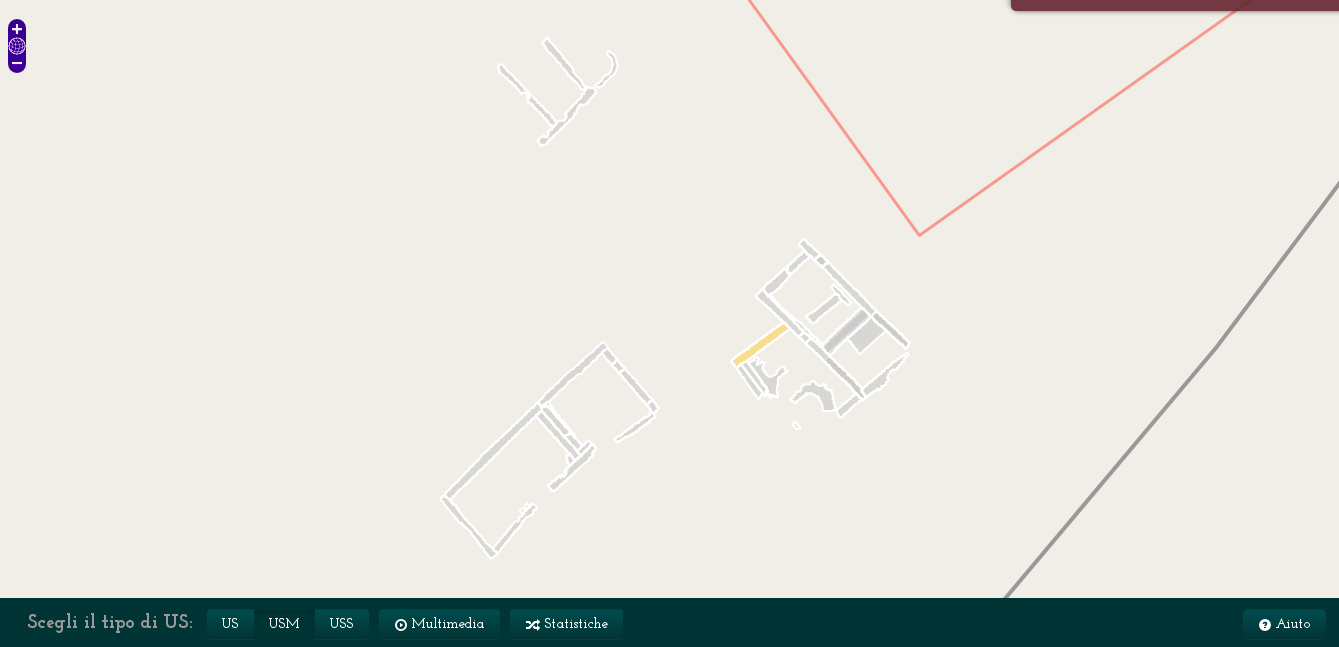
\includegraphics[width=1\linewidth]{screen_us}
				\end{center}
				\caption{Il webGIS di www.sipontoaperta.it nell'atto di mostrare le unità stratigrafiche su una carta in OpenLayers.}
				\label{fig:webgis_plain}
			\end{figure}
		\end{frame}

		\begin{frame}{Come funziona la richiesta delle voci US}
			\begin{enumerate}
				\item l'utente fa click su una delle geometrie presenti sulla mappa (US)
				\item un programmino (\emph{script}) in Python si attiva, legge le informazioni della geometria dal pacchetto dati WFS che OpenLayers conserva
				\item lo script estrapola dal WFS il codice dell'unità stratigrafica
				\item lo script si collega al database MySQL di ARK e chiede tutte le informazioni relative alla scheda con quel codice
				\item la risposta viene filtrata dallo script usando Jinja2 e viene inviata alla barra laterale, che si apre
			\end{enumerate}
		\end{frame}

		\begin{frame}{Screenshot webGIS con informazioni US}
			\begin{figure}[]
				\begin{center}
					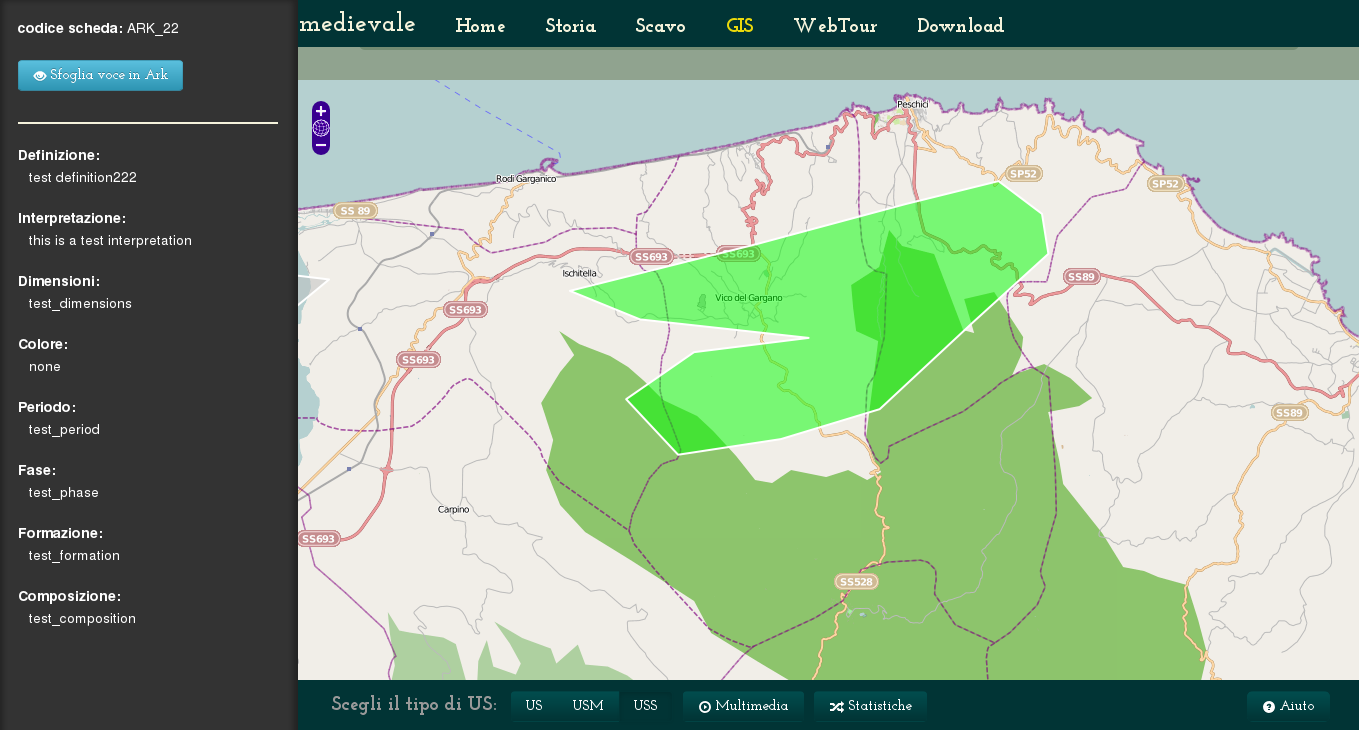
\includegraphics[width=1\linewidth]{webgis}
				\end{center}
				\caption{Il webGIS di www.sipontoaperta.it nell'atto di mostrare la scheda di US di una unità stratigrafica, selezionata sulla mappa fornita da OpenLayers.}
				\label{fig:webgis_scheda}
			\end{figure}
		\end{frame}

		\begin{frame}{Screenshot webGIS con informazioni US e layer multimediali}
			\begin{figure}[]
				\begin{center}
					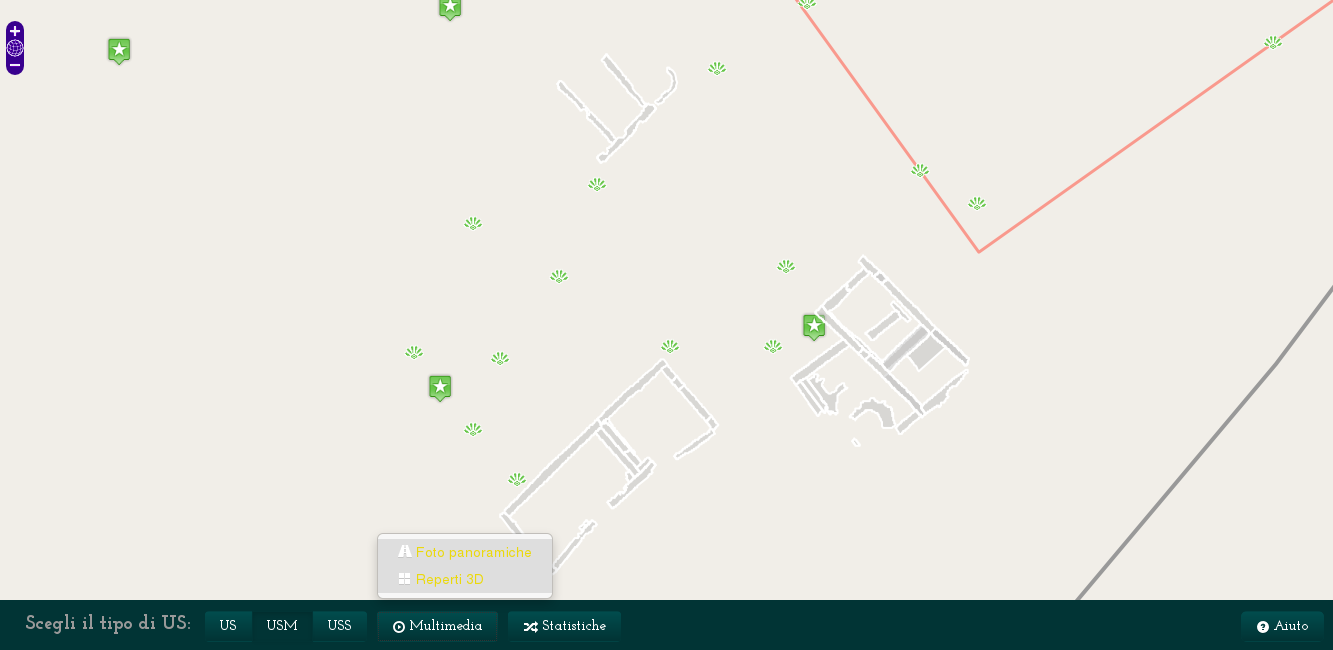
\includegraphics[width=1\linewidth]{screen_pois}
				\end{center}
				\caption{Il webGIS di www.sipontoaperta.it nell'atto di mostrare la sovrapposizione di una mappa di base, delle geometrie delle unità stratigrafiche, del layer dei punti panoramici e dei reperti 3D.}
				\label{fig:webgis_pois}
			\end{figure}
		\end{frame}

\part{Siponto Aperta: 3D}
\frame{\partpage}

	\section{Obiettivi}
		\begin{frame}{Obiettivi da progetto}
			\begin{itemize}
				\item realizzare 10 stampe 3D di altrettanti reperti sipontini
				\item rendere i modelli 3D visibili anche su web
				\item allestimento sezione per non vedenti presso Museo Scienze della Terra
			\end{itemize}
		\end{frame}
	
	\section{3D sul web}

		\begin{frame}{3D sul web}
			Punti chiave:
			\begin{itemize}
				\item dalla scansione viene ottenuta una nuvola di punti in formato .stl
				\item non esistendo uno standard per i formati 3D, non tutti i software leggono gli .stl con la stessa precisione
				\item la dimensione media di un file .stl per i reperti sipontini è di 100 mb
				\item i file devono essere fortemente ridotti prima di poter essere mostrati sul web (circa 3 mb): perdita dei dettagli
			\end{itemize}
		\end{frame}

		\begin{frame}{Thingiview}
			\begin{block}{Cos'è}
				È un software che permette di visualizzare in maniera interattiva file 3D (.stl ed altri) all'interno di una pagina web
			\end{block}
			\begin{multicols}{2}[][]
				\begin{itemize}
					\item scritto in Javascript
					\item discretamente configurabile
					\item permette di visualizzare le nuvole di punti senza scaricare tutto il file
				\end{itemize}
				\columnbreak
				\begin{figure}[]
					\begin{center}
						
\includegraphics[width=1\linewidth]{sw_logos/thingiview}
					\end{center}
					\label{fig:thingi}
				\end{figure}
			\end{multicols}
		\end{frame}

		\begin{frame}{Screenshot}
			\begin{figure}[]
				\begin{center}
					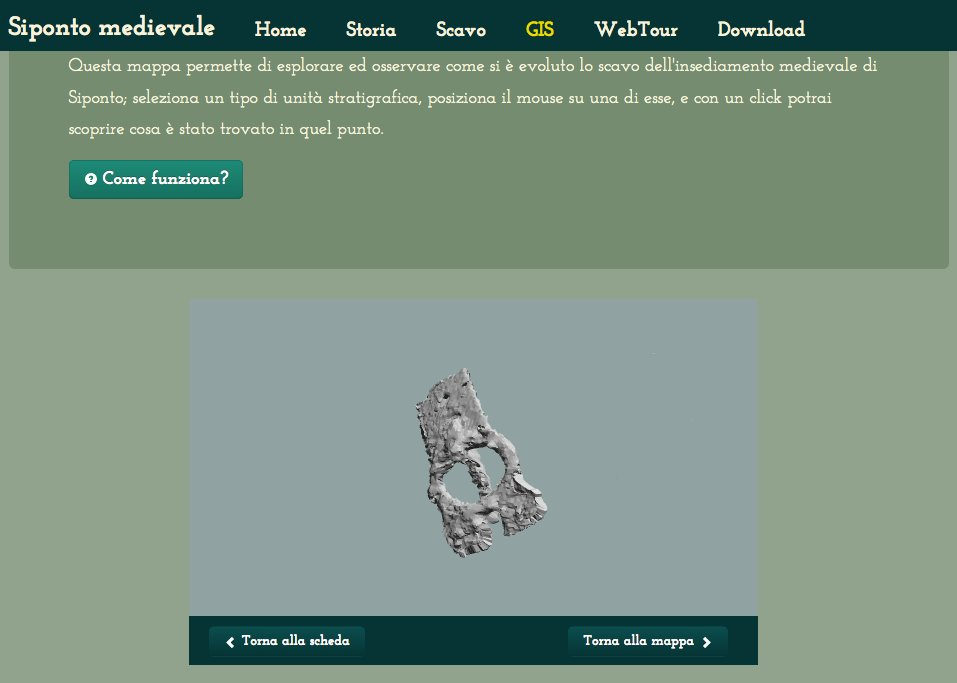
\includegraphics[width=1\linewidth]{screen_3d}
				\end{center}
				\caption{Una spilla }
			\end{figure}
		\end{frame}

		\begin{frame}
			\begin{multicols}{2}[][]
				\begin{figure}[]
					\begin{center}
						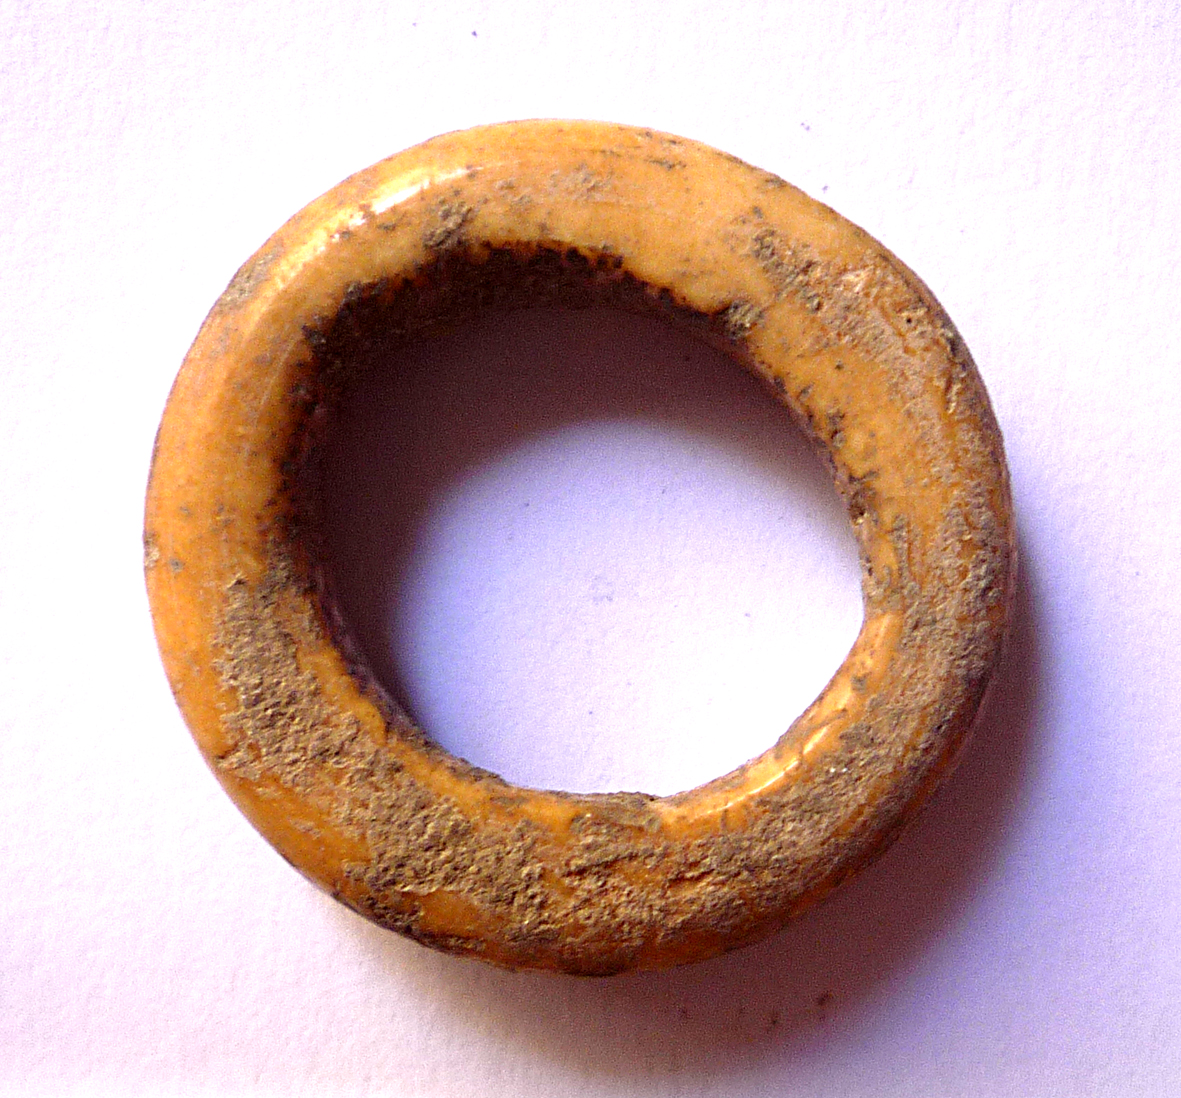
\includegraphics[width=1\linewidth]{snap3d/anello1}
					\end{center}
					\label{fig:anello1}
				\end{figure}
				\begin{figure}[]
					\begin{center}
						\includegraphics[width=1\linewidth,trim=200 0 200 0,clip=true]{snap3d/anello2}
					\end{center}
					\label{fig:anello2}
				\end{figure}
			\end{multicols}
		\end{frame}

		\begin{frame}
			\begin{multicols}{2}[][]
				\begin{figure}[]
					\begin{center}
						\includegraphics[width=1\linewidth]{snap3d/aquila1}
					\end{center}
					\label{fig:aquila1}
				\end{figure}
				\begin{figure}[]
					\begin{center}
						\includegraphics[width=1\linewidth]{snap3d/aquila2}
					\end{center}
					\label{fig:aquila2}
				\end{figure}
			\end{multicols}
		\end{frame}

		\begin{frame}
			\begin{multicols}{2}[][]
				\begin{figure}[]
					\begin{center}
						\includegraphics[width=1\linewidth]{snap3d/cane1}
					\end{center}
					\label{fig:cane1}
				\end{figure}
				\begin{figure}[]
					\begin{center}
						\includegraphics[width=1\linewidth,trim=200 0 200 0,clip=true]{snap3d/cane2}
					\end{center}
					\label{fig:cane2}
				\end{figure}
			\end{multicols}
		\end{frame}

		\begin{frame}
			\begin{multicols}{2}[][]
				\begin{figure}[]
					\begin{center}
						\includegraphics[width=1\linewidth,trim=0 200 0 0,clip=true]{snap3d/cranio1}
					\end{center}
					\label{fig:cranio1}
				\end{figure}
				\begin{figure}[]
					\begin{center}
						\includegraphics[width=1\linewidth,trim=150 0 150 0,clip=true]{snap3d/cranio2}
					\end{center}
					\label{fig:cranio2}
				\end{figure}
			\end{multicols}
		\end{frame}

		\begin{frame}
			\begin{multicols}{2}[][]
				\begin{figure}[]
					\begin{center}
						\includegraphics[width=0.7\linewidth]{snap3d/fibbia1}
					\end{center}
					\label{fig:fibbia1}
				\end{figure}
				\begin{figure}[]
					\begin{center}
						\includegraphics[width=1\linewidth,trim=150 0 150 0,clip=true]{snap3d/fibbia2}
					\end{center}
					\label{fig:fibbia2}
				\end{figure}
			\end{multicols}
		\end{frame}

		\begin{frame}
			\begin{multicols}{2}[][]
				\begin{figure}[]
					\begin{center}
						\includegraphics[width=1\linewidth,trim=50 0 250 0,clip=true]{snap3d/lucerna1}
					\end{center}
					\label{fig:lucerna1}
				\end{figure}
				\begin{figure}[]
					\begin{center}
						\includegraphics[width=1\linewidth,trim=50 0 50 0,clip=true]{snap3d/lucerna2}
					\end{center}
					\label{fig:lucerna2}
				\end{figure}
			\end{multicols}
		\end{frame}

		\begin{frame}
			\begin{multicols}{2}[][]
				\begin{figure}[]
					\begin{center}
						\includegraphics[width=1\linewidth]{snap3d/pentola1}
					\end{center}
					\label{fig:pentola1}
				\end{figure}
				\begin{figure}[]
					\begin{center}
						\includegraphics[width=1\linewidth,trim=230 0 200 0,clip=true]{snap3d/pentola2}
					\end{center}
					\label{fig:pentola2}
				\end{figure}
			\end{multicols}
		\end{frame}

		\begin{frame}
			\begin{multicols}{2}[][]
				\begin{figure}[]
					\begin{center}
						\includegraphics[width=1\linewidth]{snap3d/vaso1}
					\end{center}
					\label{fig:vaso1}
				\end{figure}
				\begin{figure}[]
					\begin{center}
						\includegraphics[width=1\linewidth,trim=50 0 230 0,clip=true]{snap3d/vaso2}
					\end{center}
					\label{fig:vaso2}
				\end{figure}
			\end{multicols}
		\end{frame}
\end{document}
